\documentclass{beamer}

\mode<presentation> {

% The Beamer class comes with a number of default slide themes
% which change the colors and layouts of slides. Below this is a list
% of all the themes, uncomment each in turn to see what they look like.

%\usetheme{default}
%\usetheme{AnnArbor}
%\usetheme{Antibes}
%\usetheme{Bergen}
%\usetheme{Berkeley}
%\usetheme{Berlin}
%\usetheme{Boadilla}
%\usetheme{CambridgeUS}
%\usetheme{Copenhagen}
%\usetheme{Darmstadt}
%\usetheme{Dresden}
\usetheme{Frankfurt}
%\usetheme{Goettingen}
%\usetheme{Hannover}
%\usetheme{Ilmenau}
%\usetheme{JuanLesPins}
%\usetheme{Luebeck}
%\usetheme{Madrid}
%\usetheme{Malmoe}
%\usetheme{Marburg}
%\usetheme{Montpellier}
%\usetheme{PaloAlto}
%\usetheme{Pittsburgh}
%\usetheme{Rochester}
%\usetheme{Singapore}
%\usetheme{Szeged}
%\usetheme{Warsaw}

% As well as themes, the Beamer class has a number of color themes
% for any slide theme. Uncomment each of these in turn to see how it
% changes the colors of your current slide theme.

%\usecolortheme{albatross}
%\usecolortheme{beaver}
%\usecolortheme{beetle}
\usecolortheme{crane}
%\usecolortheme{dolphin}
%\usecolortheme{dove}
%\usecolortheme{fly}
%\usecolortheme{lily}
%\usecolortheme{orchid}
%\usecolortheme{rose}
%\usecolortheme{seagull}
%\usecolortheme{seahorse}
%\usecolortheme{whale}
%\usecolortheme{wolverine}

%\setbeamertemplate{footline} % To remove the footer line in all slides uncomment this line
%\setbeamertemplate{footline}[page number] % To replace the footer line in all slides with a simple slide count uncomment this line

%\setbeamertemplate{navigation symbols}{} % To remove the navigation symbols from the bottom of all slides uncomment this line
}

\usepackage{extpfeil}
\usepackage{extarrows} %Allows long equation signs
\usepackage{graphicx} % Allows including images
\usepackage{booktabs} % Allows the use of \toprule, \midrule and \bottomrule in tables
\usepackage{physics}
\usepackage{tikz}
\usepackage{cite}
%花体字母
\usepackage{amsthm,amsmath,amssymb}
\usepackage{mathrsfs}
\usepackage{dutchcal}
\usepackage{circuitikz}

%----------------------------------------------------------------------------------------
%	TITLE PAGE
%----------------------------------------------------------------------------------------

\title[VP260 RC]{Midterm Review} % The short title appears at the bottom of every slide, the full title is only on the title page

\author{VP260 TA Group} % Your name
\institute[UM-SJTU JI] % Your institution as it will appear on the bottom of every slide, may be shorthand to save space
{
    University of Michigan - Shanghai Jiao Tong University Joint Institute\\% Your institution for the title page
\medskip
}
\date{\today} % Date, can be changed to a custom date

\AtBeginSection[]
{
  \begin{frame}
    \frametitle{Table of Contents}
    \tableofcontents[currentsection]
  \end{frame}
}

\begin{document}

\begin{frame}
    \titlepage % Print the title page as the first slide
\end{frame}

\begin{frame}{Outline}
\tableofcontents
\end{frame}

%----------------------------------------------------------------------------------------
%	 SECTION 1
%----------------------------------------------------------------------------------------
\section{Fundamental Concepts}

\subsection{Vector Calculus} % Section title slide, unnumbered

\begin{frame}{Stoke's formula}
	\begin{block}{Foundamental theorem for gradients}
		\begin{equation}
			\int_{\vb{a}}^{\vb{b}} (\grad f) \vdot \dd{\vb*{l}} = f(\vb{b}) - f(\vb{a})
		\end{equation}
	\end{block}
	
	\begin{block}{Divergence theorem}
		\begin{equation}
			\int_V (\div \vb{v}) \dd{\tau} = \oint_{\partial V} \vb{v} \vdot \dd{\vb*{A}}
		\end{equation}
	\end{block}

	\begin{block}{Stoke's theorem}
		\begin{equation}
			\int_S (\curl \vb{v}) \vdot \dd{\vb{A}} = \oint_{\partial S} \vb{v} \vdot \dd{\vb{l}}
		\end{equation}
	\end{block}
\end{frame}

\subsection{Electrostatics}

\begin{frame}{Electric Field}	
	\begin{block}{Coulomb Force}
		\begin{equation}
			\vec{F} = \frac{1}{4\pi\epsilon_0} \frac{\abs{q_1 q_2}}{r^2} \vu{r}
		\end{equation}	
    \end{block}

    \begin{block}{Electric Field}
        \begin{equation}
			\vec{E} = \frac{\vec{F}}{q_0}
		\end{equation}
    \end{block}
    
    \begin{block}{Electric potential}
        \begin{equation}
            V(\va{r}) = -\int_O^{\va{r}} \va{E} \vdot \dd{\va{l}}
        \end{equation}
    \end{block}

	\begin{itemize}
        \item Superposition principle.
	\end{itemize}
\end{frame}


\begin{frame}{Gauss' Law}
	\begin{beamerboxesrounded}{Electric flux}
		\begin{equation}
			\Phi_E = \int_{S} \va{E} \vdot \dd{\va{A}}
		\end{equation}
	\end{beamerboxesrounded}
	\vspace{1em}
	\begin{beamerboxesrounded}{Gauss' law}
		\begin{equation}
			\oint_{S} \va{E} \cdot \dd{\va{A}} = \frac{q_{enc}}{\epsilon_0}
		\end{equation}
		\begin{equation}
			\div \va{E} = \frac{\rho(\vec{r})}{\epsilon_0}
		\end{equation}
	\end{beamerboxesrounded}
	\begin{itemize}
		\item The $q_{enc}$ is the total charge enclosed in the surface.
	\end{itemize}
\end{frame}


\begin{frame}{Potential energy}
    Move a test charge $q$ from point $\va{a}$ to $\va{b}$, the minimum work is,
    \begin{equation}
        W = \int_{\vb{a}}^{\vb{b}} \va{F} \vdot \dd{\va{l}} = -q \int_{\vb{a}}^{\vb{b}} \va{E} \vdot \dd{\va{l}} = q \cdot (V(\va{b}) - V(\va{a}))
    \end{equation}

    \begin{block}{Potential energy}
        \begin{equation}
            U(\va{r}) = q \cdot V(\va{r})
        \end{equation}
    \end{block}

    \begin{itemize}
        \item The minimum work for moving a test charge $q$ from point $\va{a}$ to $\va{b}$ is $U(\va{b}) - U(\va{a})$.
    \end{itemize}
\end{frame}


\begin{frame}{Configuration Energy}
    Discrete distribution,
    \begin{equation}
        U_{conf} = \frac{1}{8 \pi \epsilon_0} \sum_{i} \sum_{j, i \neq j} \frac{q_i q_j}{r_{ij}} = \frac{1}{2} \sum_{i} q_i V(\va{r_i}).
    \end{equation}

    Continuous distribution,
    \begin{equation}
        U_{conf} = \frac{1}{2} \int_{\Omega} \rho V \dd{\tau} = \frac{\epsilon_0}{2} \left( \oint_{\Sigma} V \va{E} \vdot \dd{\va{A}} + \int_{\Omega} E^2 \dd{\tau} \right).
    \end{equation}

    For the whole space,
    \begin{equation}
        U_{conf} = \frac{\epsilon_0}{2} \int_{\mathbb{R}^3} E^2 \dd{\tau}.
    \end{equation}
\end{frame}


\begin{frame}{Conductor}
    \begin{itemize}
        \item Electric field lines is perpendicular to equipotential surfaces;
        \item The surface of a conductor is equipotential (electrostatic).
    \end{itemize}
    \vspace{1em}
    \begin{beamerboxesrounded}[shadow=true]{Properties of Conductors}
        \begin{itemize}
            \item $\va{E} = 0$ \textbf{everywhere} inside a conductor;
            \item Any excess charge placed on a conductor resides entirely on its surface;
            \item Any conductor is equipotential.
        \end{itemize}
    \end{beamerboxesrounded}
\end{frame}


\begin{frame}{Electric Field}
    \begin{block}{Toolbox for calculating electric field}
        \begin{itemize}
            \item $\va{E} = \div{V}$;
            \item Add up contributions from small charges dq regarded as point charges;
            \item Use Gauss's law (symmetry).
        \end{itemize}
    \end{block}
\end{frame}

\begin{frame}{Electric Potential}
    \begin{block}{Conservative field}
        \begin{equation}
            \oint_l \va{E} \vdot \dd{\va{s}} = 0
        \end{equation}
        \begin{equation}
            \curl{\va{E}} = 0
        \end{equation}
    \end{block}

    \begin{block}{Toolbox for calculating potential}
        \begin{itemize}
            \item $V(\va{r}) = -\int_O^{\va{r}} \va{E} \vdot \dd{\va{l}}$;
            \item Add up contributions from small charges dq regarded as point charges;
            \item Solve equation $- \laplacian{V} = \frac{\rho}{\epsilon_0}$ with boundary condition (method of image).
        \end{itemize}
    \end{block}
\end{frame}


\begin{frame}{Method of Image}
    \begin{block}{Poisson's Equation (PDE)}
        \begin{equation}
            - \laplacian{V} = \frac{\rho}{\epsilon_0}
        \end{equation}
    \end{block}

    \begin{block}{Uniqueness theory}
        The electric potential inside a certain is \textbf{uniquely} determined, if:
        \begin{itemize}
            \item Charge density $\rho$ throughout the domain $\Omega$ is known
            \item The electric potential distribution at the boundaries is known
        \end{itemize}
    \end{block}

    \begin{block}{Method of Images}
        Add mirror images \textbf{outside} the original domain, to satisfy the boundary conditions.
    \end{block}
    
\end{frame}

\begin{frame}{Summary for Electrostatics}
    \begin{figure}[htbp]
        \centering
        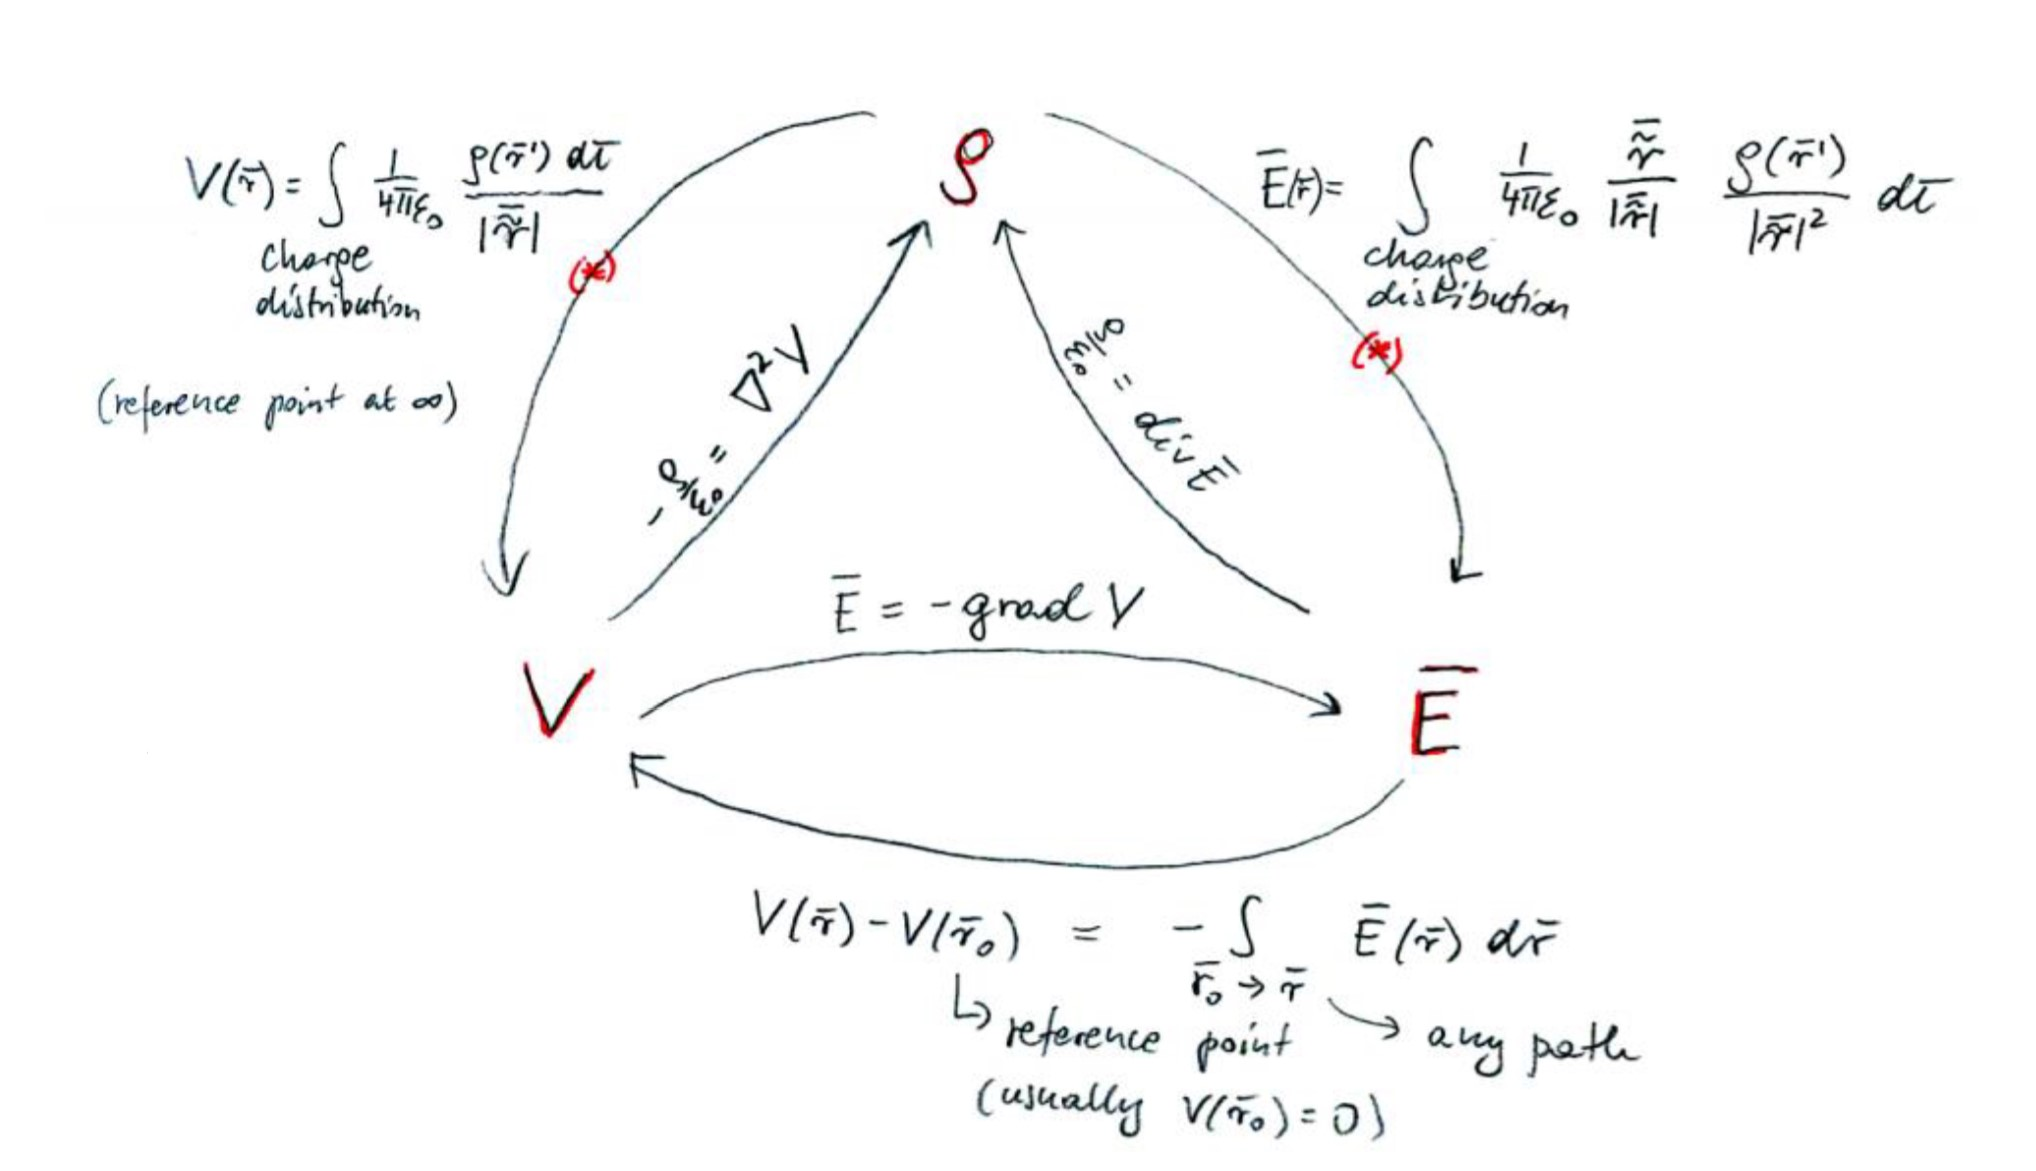
\includegraphics[width=\textwidth]{images/elec.jpg}
    \end{figure}
\end{frame}

%------------------------------------------------

\subsection{DC Circuit}

\begin{frame}{Capacitor \& Capacitance}
    \begin{beamerboxesrounded}[shadow=true]{Capcitance}
        \begin{equation}
            C = \frac{Q}{V_{ab}}
        \end{equation}
    \end{beamerboxesrounded}
    \begin{itemize}
        \item Unit: $1F = 1C/1V$
        \item $V_{ab} = V_a - V_b$
    \end{itemize}

    \begin{beamerboxesrounded}[shadow = true]{Energy}
        \begin{equation}
            U = W = \frac{Q^2}{2C} = \frac{1}{2} CV^2 
        \end{equation}
    \end{beamerboxesrounded}

    \begin{block}{Energy density}
        \begin{equation}
            u = \frac{1}{2} \epsilon_0 E^2
        \end{equation}
    \end{block}     
\end{frame}


\begin{frame}{Dielectrics}
    \begin{itemize}
        \item Relative permittivity: $ \epsilon_r $
        \item Absolute permittivity: $ \epsilon = \epsilon_r \epsilon_0$
    \end{itemize}
    \vfill
    \begin{block}{Gauss's law}
        \begin{equation}
            \oint_S \va{E} \vdot \dd{\va{A}} = \frac{Q_{encl}}{\epsilon_0}
        \end{equation}
        \begin{equation}
            \oint_S \epsilon_r \va{E} \vdot \dd{\va{A}} = \frac{Q_{free-encl}}{\epsilon_0}
        \end{equation}
    \end{block}
    \begin{beamerboxesrounded}[shadow=true]{Formulas with dielectrics}
        \begin{equation}
            \left\{
                \begin{array}{ll}
                    \vspace{.5em}
                   & V = \frac{V_0}{\epsilon_r} \\ \vspace{.5em}
                   & E = \frac{E_0}{\epsilon_r} = \frac{\sigma}{\epsilon} \\ \vspace{.5em}
                   & C = \epsilon \frac{A}{d} \\\vspace{.5em}
                   & u = \frac{1}{2} \epsilon E^2
                \end{array}
            \right.
        \end{equation}
    \end{beamerboxesrounded}    
\end{frame}

\begin{frame}{Electric Current}
    \begin{beamerboxesrounded}[shadow=true]{Current density}
        \begin{equation}
            \begin{array}{llll}
               & \va*{J} &=& qn\va*{v_d} \vspace{.6em}\\
               & \abs*{\va*{J}} &=& \frac{I}{A}
            \end{array}
        \end{equation}
    \end{beamerboxesrounded}
    \vfill
    \begin{beamerboxesrounded}[shadow=true]{Ohm's law (microscopic form)}
        \begin{equation}
            \begin{split}
                \va*{J} &= \sigma \va*{E} \\
                \va*{J} &= \frac{\va*{E}}{\rho}
            \end{split}
        \end{equation}
    \end{beamerboxesrounded}
\end{frame}

\begin{frame}{Kirchhoff's Rule}
    \begin{block}{Kirchhoff's rule}
        \begin{itemize}
            \item Junction rule (KCL):
                \begin{equation}
                    \sum_k I_k = 0
                \end{equation}
                where $I_k$ represents a current flows into the junction.
            \item Loop rule (KVL):
                \begin{equation}
                    \sum_k V_k = 0
                \end{equation}
                where $V_k$ represents the voltage across the element in a loop
        \end{itemize}.
    \end{block}
\end{frame}

\begin{frame}{Direct Current RC Circuits}
    \begin{columns}
        \begin{column}{.5\linewidth}
            \begin{block}{Charging}
                \begin{center}
                    \begin{circuitikz}
                        \draw (0,0) to[battery1=$\epsilon$] (4,0) -- (4,2) to[R=$R$](2,2) -- (1.5,2) to[C=$C$] (0,2) -- (0,0);
                    \end{circuitikz}
                \end{center}
            \end{block}
        \end{column}

        \begin{column}{.5\linewidth}
            \begin{block}{Discharging}
                \begin{center}
                    \begin{circuitikz}
                        \draw (0,0) to[R=$R$] (4,0) -- (4,2) to[C=$C$] (0,2) -- (0,0);
                    \end{circuitikz}
                \end{center}
            \end{block}
        \end{column}
    \end{columns}
\end{frame}


\subsection{Magnetic field}

\begin{frame}{Magnetic Force}
    \begin{block}{Lorentz force}
        \begin{equation}
            \va{F} = q (\va{v} \crossproduct \va{B})
        \end{equation}
    \end{block}
    \begin{itemize}
        \item Magnetic forces do no work.
    \end{itemize}
    \vfill
    \begin{block}{Ampere's force}
        The magnetic force on a segment of current-carrying wire is,
        \begin{equation}
            \va{F} = \int I (\dd{\va{l} \crossproduct \va{B}})
        \end{equation}
    \end{block}
\end{frame}


\begin{frame}{Magnetic Fluxa and Gauss' Law}
    \begin{block}{Magnetic flux}
        \begin{equation}
            \Phi_B = \int_\Sigma \va{B} \vdot \dd{\va{A}}
        \end{equation}
    \end{block}
    \begin{itemize}
        \item Unit: Weber [Wb]
    \end{itemize}
    \vfill
    \begin{block}{Gauss' law for the magnetic field}
        For any closed surface $\Sigma$,
        \begin{equation}
            \Phi_B = \oint_\Sigma \va{B} \vdot \dd{\va{A}} = 0
        \end{equation}
        Hence,
        \begin{equation}
            \div{\va{B}} = 0
        \end{equation}
    \end{block}
\end{frame}



%----------------------------------------------------------------------------------------
%	 Section 2
%----------------------------------------------------------------------------------------

\section{Exercise}

\subsection{\bf Electric Field \& Gauss' Law}

\begin{frame}{\bf Hw2 P2}
A point charge $q$ is placed at the point $\mathbf{r}=0$.
(a) By direct calculation show that the divergence of the 
electric field $\operatorname{div} \mathbf{E}(\mathbf{r})=0$ 
for all $\mathbf{r} \neq 0 .$ What can you say (qualitatively) 
about the divergence at $\mathbf{r}=0 ?$
(b) What is the condition $\operatorname{div} \mathbf{E}(\mathbf{r})$ 
should satisfy at $\mathbf{r}=0$ for Gauss's law to be valid? 
\end{frame}

\begin{frame}{\bf Hw2 P9}
    \begin{columns}
        \begin{column}{.7\linewidth}
            Two spherical cavities, of radii $r_{a}$ and $r_{b}$, are hollowed out from the interior of a neutral conducting ball of radius $R$. At the center of each cavity a point charge is placed: $q_{a}$ and $q_{b},$ respectively.
            (a) Find the surface densities of charge $\sigma_{a}, \sigma_{b}$ on the walls of the cavities as well as on the surface of the ball $\sigma_{R}$.
            (b) What is the electric field outside of the conductor?
            (c) What is the electric field within each cavity?
            (d) What is the force on $q_{a}$ and $q_{b} ?$
            (e) Which of these answers would change if a third charge $q_{c}$ were brought near the conductor?

        \end{column}
        \begin{column}{.3\linewidth}
            \begin{figure}
                \centering
                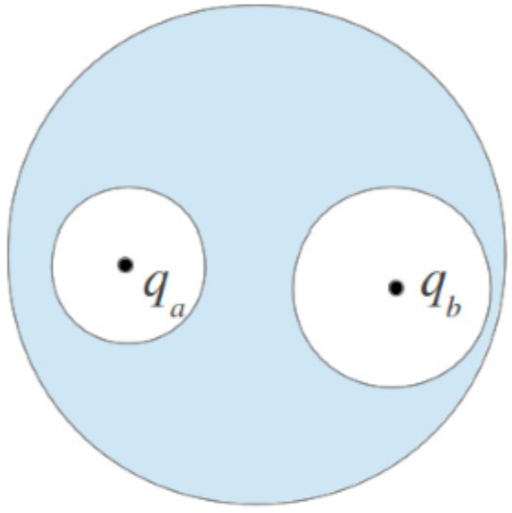
\includegraphics[scale=0.4]{images/ex2.png}
            \end{figure}
        \end{column}
    \end{columns}

\end{frame}

\begin{frame}{\bf Hw3 P3}
    What is the electric potential at a distance $s$ from an infinitely long straight wire charged with uniform density $\lambda$ ? Comment on your choice of the reference point.
\end{frame}

\begin{frame}{\bf Hw3 P4}
    A conical surface (an empty ice-cream cone) carries a uniform surface charge with density $\sigma$. The height of the cone is $h,$ as is the radius of the top. Find the electric potential difference between points $\mathbf{r}_{A}$ (the vertex) and $\mathbf{r}_{B}$ (the center of the top).
\end{frame}


\begin{frame}{\bf Exercise 1}
There are two positive point charges $q_1$ and $q_2$ locating at 
$r_1$ and $r_2$ respectively. Now add a negative point charge $q_3$ 
into the system. Please find out where it should be put and 
what its magnitude is so that the electric forces exerted on 
all three charges equal to 0.

\begin{figure}[htbp]
    \centering
    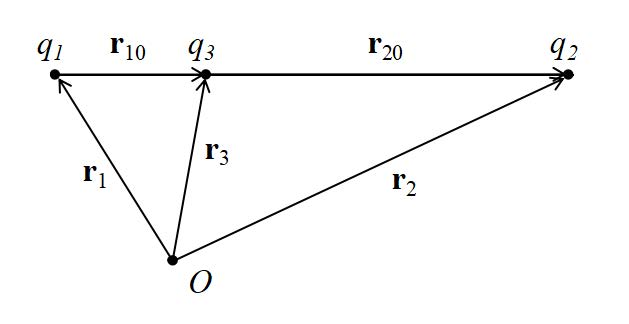
\includegraphics[scale = 0.8]{images/EF_1.jpg}
\end{figure}
\end{frame}


\begin{frame}{\bf Exercise 2}
There is a metal ball ($R$, $Q$) in space. Calculate the force between the upper and lower half balls.

\begin{figure}[htbp]
    \centering
    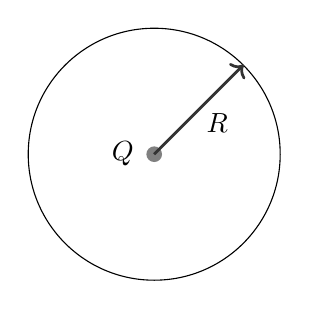
\begin{tikzpicture}[scale=0.8]
        \draw (0,0) circle (2);
        \node[circle,fill = black!50,inner sep =2pt] () at (0,0) {};
        \node[] () at (-0.5,0) {$Q$};
        \node[] () at (1,0.5) {$R$};
        \draw[->, line width = .035cm, black!80] (0,0) -- (1.42,1.42);
    \end{tikzpicture}
\end{figure}
\end{frame}

\subsection{\bf Electric Potential}

\begin{frame}{\bf Hw3 P7}
    Find the energy stored in a uniformly charged solid ball of radius $R$ and charge $q$. (This energy is also often called the "self-energy" of the charge distribution.) Do it in four different ways, using formulas we have derived in class:
(a) Use $U_{\text {conf }}=\frac{1}{2} \int_{\Omega} \rho V d \tau$. \\
(b) Use $U_{\text {conf }}=\frac{\varepsilon_{0}}{2} \int_{\text {all space }} E^{2} d \tau$. \\
(c) Use $U_{\text {conf }}=\frac{\varepsilon_{0}}{2}\left(\int_{\Omega} E^{2} d \tau+\oint_{\Sigma} V \mathbf{E} \circ d \mathbf{A}\right)$ taking $\Sigma$ as a sphere of radius $a>R$ centered at the center of the ball. Comment on what happens as $a \rightarrow \infty$. \\
(d) Find the amount of work needed to be done to assemble the ball by bringing infinitesimal charges from far away. 
\end{frame}

\begin{frame}{\bf Exercise 3}
    \begin{columns}
        \begin{column}{0.6\linewidth}
        There are three point charges with mass \textit{m} and positive charge \textit{q}. Initially, they stay still 
        at three vertexes of an equilateral triangle with side length \textit{l} and there is a rigid insulating rod connecting each 
        point charge. Point \textit{C} is the center of the equilateral triangle. Now cut the rod between point charges 1 and 2, please find out:\\
        (1) When point charge 3 reaches \textit{C}, what is its speed?\\
        (2) During the entire process, what is the maximum speed of point charge 3?
        \end{column}
        \begin{column}{.4\linewidth}
            \begin{figure}[H]
                \centering
                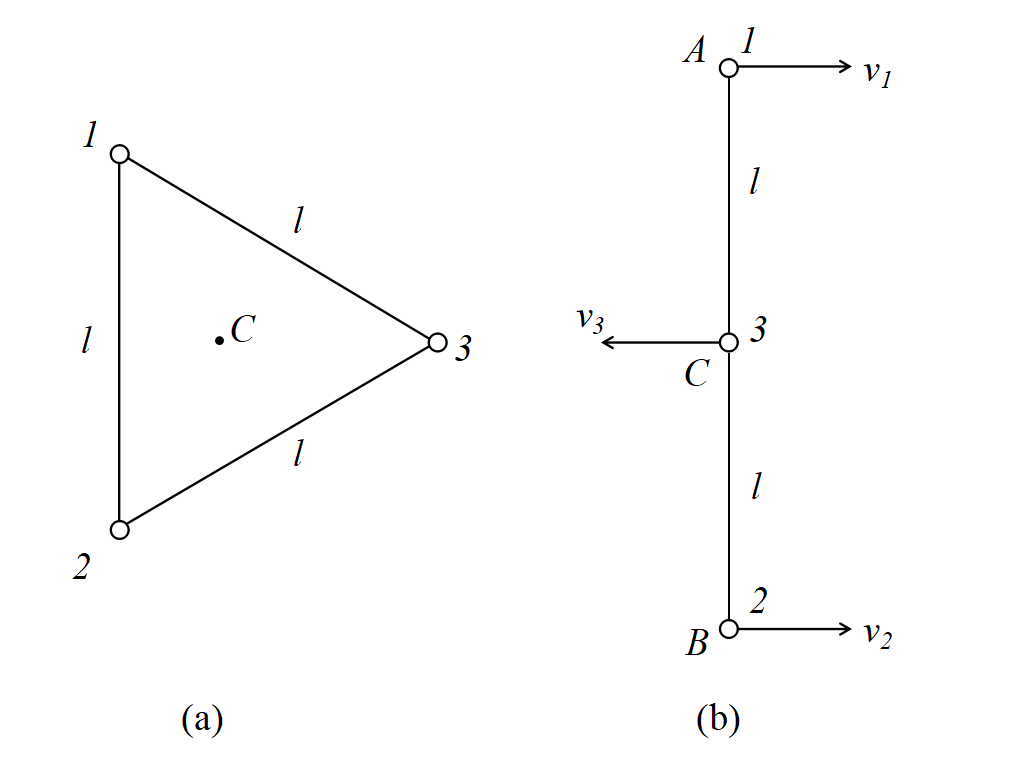
\includegraphics[scale=0.4]{images/009.png}
                \end{figure}
        \end{column}
    \end{columns}
\end{frame}


\begin{frame}{\bf Exercise 4}
    Please first judge the following statement and then give your proof:\\
    If a solid (means not hollow here) conductor carries a total charge of +\textit{Q} ($Q<0$), 
    then the surface charge density $\sigma$ is greater than or equal to 0 everywhere on the surface of the conductor.
\end{frame}

%------------------------------------------------------%

\subsection{\bf Method of Image}


\begin{frame}{\bf Hw4 P5}
    
(a) Calculate the electric potential in this region. 
(b) What is the force on q? (c) How much work did it take to bring the charge q from infinity? 
(d) For what particular angles does the method work?
    
\begin{figure}
    \centering
    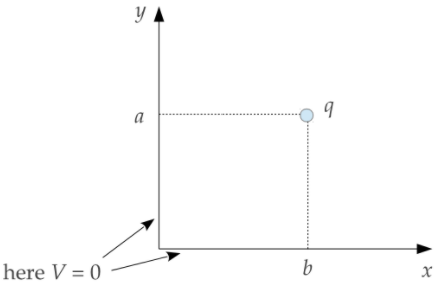
\includegraphics[scale=0.75]{images/ex5.png}
\end{figure}

\end{frame}


\begin{frame}{\bf Exercise 5 (RC 2)}
    There exists a point charge $Q$ and a conducting shell in space. The distance between the center of shell 
    and the point charge is $a(a>R_0)$. Please find out the total amount of induced charge on the surface, in each case:
    \begin{itemize}
        \item The conducting shell is grounded
        \item The conducting shell is neither grounded nor carrying any charge at first
        \item The conducting shell is not grounded but at an electric potential $V_0$
        \item The conducting shell is not grounded but carrying charge $q$ at first
        \item What if $a<R_0$?
    \end{itemize}
\end{frame}

%---------------------------------------------------%

\subsection{\bf Capacitors}

\begin{frame}{\bf Hw4 8}
    Two square conducting plates with sides of length $L$ are separated by a distance $D$. A dielectric slab with relative permittivity $\varepsilon_{\mathrm{r}}$ and dimensions $L \times L \times D$ is inserted a distance $x$ into the space between the plates, as shown in the figure.
    \begin{figure}
        \centering
        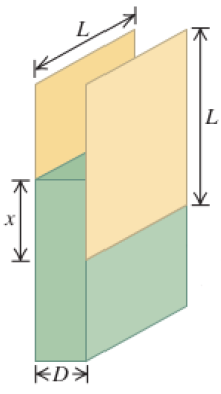
\includegraphics[scale=0.8]{images/HW4_8}
    \end{figure}
\end{frame}

\begin{frame}{\bf Exercise 6}
    Two metal boards are placed parallel to each other and 
    separated at a distance $D=2cm$. The surface charge density 
    on one board is $\sigma_{1}=3\mu C/m^2$ and $\sigma_{2}=6\mu C/m^2$ 
    for another. A wax board with thickness $D/2$ whose relative 
    permittivity is $\varepsilon_{r}=2$ is placed between two boards. 
    Please find out the potential difference between two boards.
\begin{figure}
    \centering
    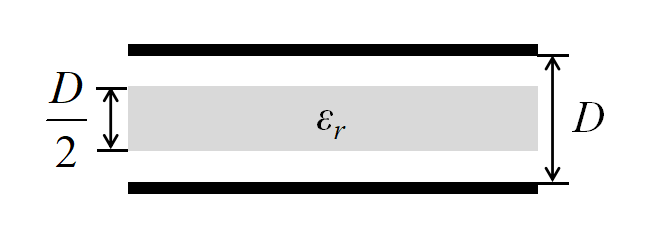
\includegraphics[scale=0.6]{images/013.png}
\end{figure} 

\end{frame}

\begin{frame}{\bf Exercise 7}
\begin{columns}
    \begin{column}{.7\linewidth}
        A parallel-plane capacitor is inserted into a beaker containing liquid dielectric with relative permittivity $\varepsilon_{r}$ and density $\rho$. 
        Assume that the surface area of the plane is $S$ (with height $h$ and width $a$). The distance between two planes is $d$. There is an external power 
        source to maintain the voltage across the capacitor at $V$. Given that the acceleration due to gravity is $g$, please find out the rise of liquid dielectric in the capacitor $h$.
    \end{column}
    \begin{column}{.3\linewidth}
        \begin{figure}
            \centering
            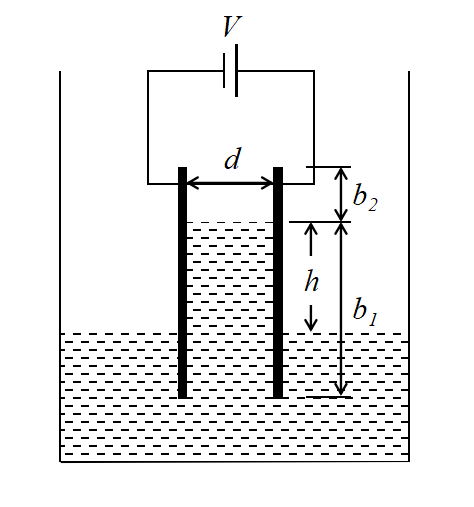
\includegraphics[scale=0.6]{images/014.png}
        \end{figure}
    \end{column}
\end{columns}
\end{frame}


%-------------------------------------------%
\subsection{\bf Electric Current}

\begin{frame}{\bf Hw5 P1}
    \begin{columns}
        \begin{column}{.7\linewidth}
            Two concentric spherical metal shells with radii $r_{a}, r_{b},$ 
            where $r_{a}<r_{b},$ are separated by a weakly conducting material 
            with conductivity $\sigma$. \\
            (a) If they are maintained at potential difference $V,$ what current flows from one to each other? \\
            (b) What is the resistance between the shells? \\ 
            (c) Notice that if $r_{b} \gg r_{a},$ the outer radius $r_{b}$ is irrelevant. Determine the current flowing between two metal spheres, each of radius $r_{a}$, immersed deep in the sea and held quite far apart, if the potential difference between them is $V$.
        \end{column}
        \begin{column}{.3\linewidth}
            \begin{figure}
                \centering
                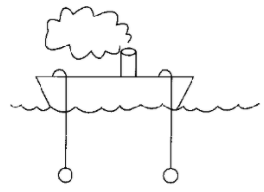
\includegraphics[scale=0.8]{images/HW5_1.png}
            \end{figure}
        \end{column}
    \end{columns}
\end{frame}

\begin{frame}{\bf Hw5 P2}
    Estimate the resistance between the wires.
    \vspace{1em}
    \begin{figure}
        \centering 
        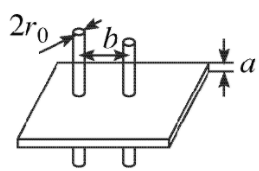
\includegraphics[scale = 1]{images/HW5_2.png}
    \end{figure}
\end{frame}


\begin{frame}{\bf Exercise 8}
    There are two concentric metal spheres with radius $a$ 
    and $b$ respectively ($b>a$). There are materials with 
    conductivity $\sigma=KE$ where $K$ is a positive constant 
    and $E$ is the magnitude of the electric field. Now 
    maintain the electric potential difference between 
    two spheres at $V$, please find out the current flowing 
    between two spheres.
\end{frame}


%---------------------------------------------%

\subsection{\bf Magnetic Field}

\begin{frame}{\bf Exercise 9}
    A simple pendulum consists of a string with length $L$ 
    and a ball carrying charge $+q$. The greatest swing angle is $\alpha$. 
    In order to make this pendulum oscillate normally, what kind of restrict 
    must be placed on the magnitude of the magnetic field?

    \begin{figure}
        \centering
        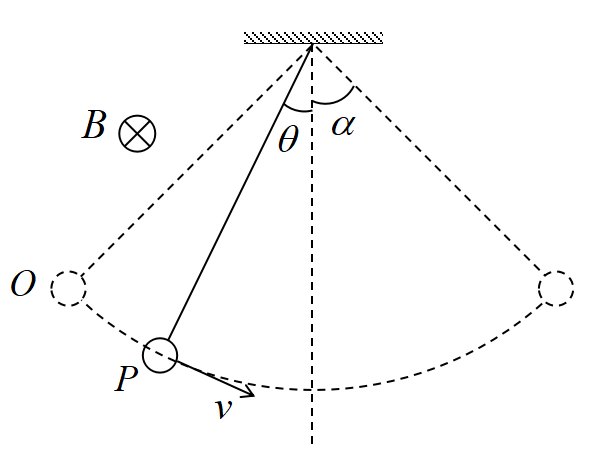
\includegraphics[scale=0.6]{images/005.png}
    \end{figure}
\end{frame}

\begin{frame}{\bf Exercise 10}
    There is a particle with mass m and charge $+q$ shot from point $a$ 
    with a initial velocity $v_0$ pointing straightly towards point $b$. 
    If the particle can exactly pass through point $b$, what are the possible 
    values of the magnitude of $v_0$? (consider the gravitational force)

    \begin{figure}
        \centering 
        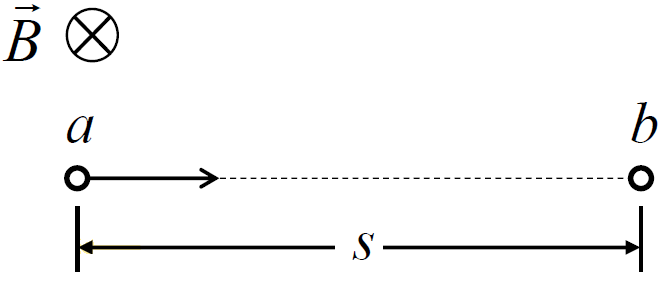
\includegraphics[scale=0.5]{images/Ex11.png}
    \end{figure}
\end{frame}


%-----------------------------------------------%
\subsection{\bf Ampere's Force}
\begin{frame}{\bf Exercise 11}
    $m_ab=5$g, $h=0.8$m, $L_ab=1$m, $C=400\mu$F, $\varepsilon=16$V, $B=0.5$T. 
    The switch $S$ is first at position 1 for a long enough time, 
    then suddenly moved to position 2. The metal bar will be 
    catapulted to the ground and cover a horizontal distance 
    $x=6.4$cm. Neglect the air drag and any friction, and given that the 
    acceleration due to gravity $g=10$m/s$^{2}$, please 
    find out the voltage across the capacitor after the 
    metal bar is catapulted.

    \begin{figure}[H]
        \centering
        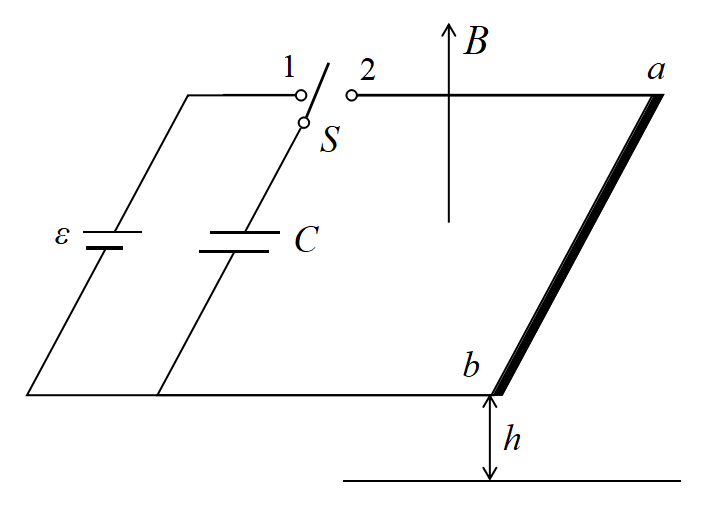
\includegraphics[scale=0.45]{images/007.png}
    \end{figure}
\end{frame}


%----------------------------------------------------------------------------------------
%	 CLOSING/SUPPLEMENTARY SLIDES
%----------------------------------------------------------------------------------------

\begin{frame}
    \begin{center}
        \LARGE\bf LALALA
    \end{center}
	
\end{frame}


\section*{Appendix}

%----------------------------------------------------------------------------------------

\begin{frame}{\bf References}
	\nocite{*} % Display all references regardless of if they were cited
	\bibliography{example.bib}
	\bibliographystyle{plain}
\end{frame}

\end{document}

